\chapter{User Interface Specification}

% This section contains mockups, descriptions,
% and explanations, lots of graphics
\section{Preliminary Design}

\subsection{Company}
From this page, you are able to view details statistics about certain companies after being linked to it or searching for it. Major details, such as the quote, are up at the top while further details are at the bottom. A user can comment on the company on the bottom right. If you decide that you want to trade, you simply press the trade button and a box will pop-up, giving you options for the trade.//
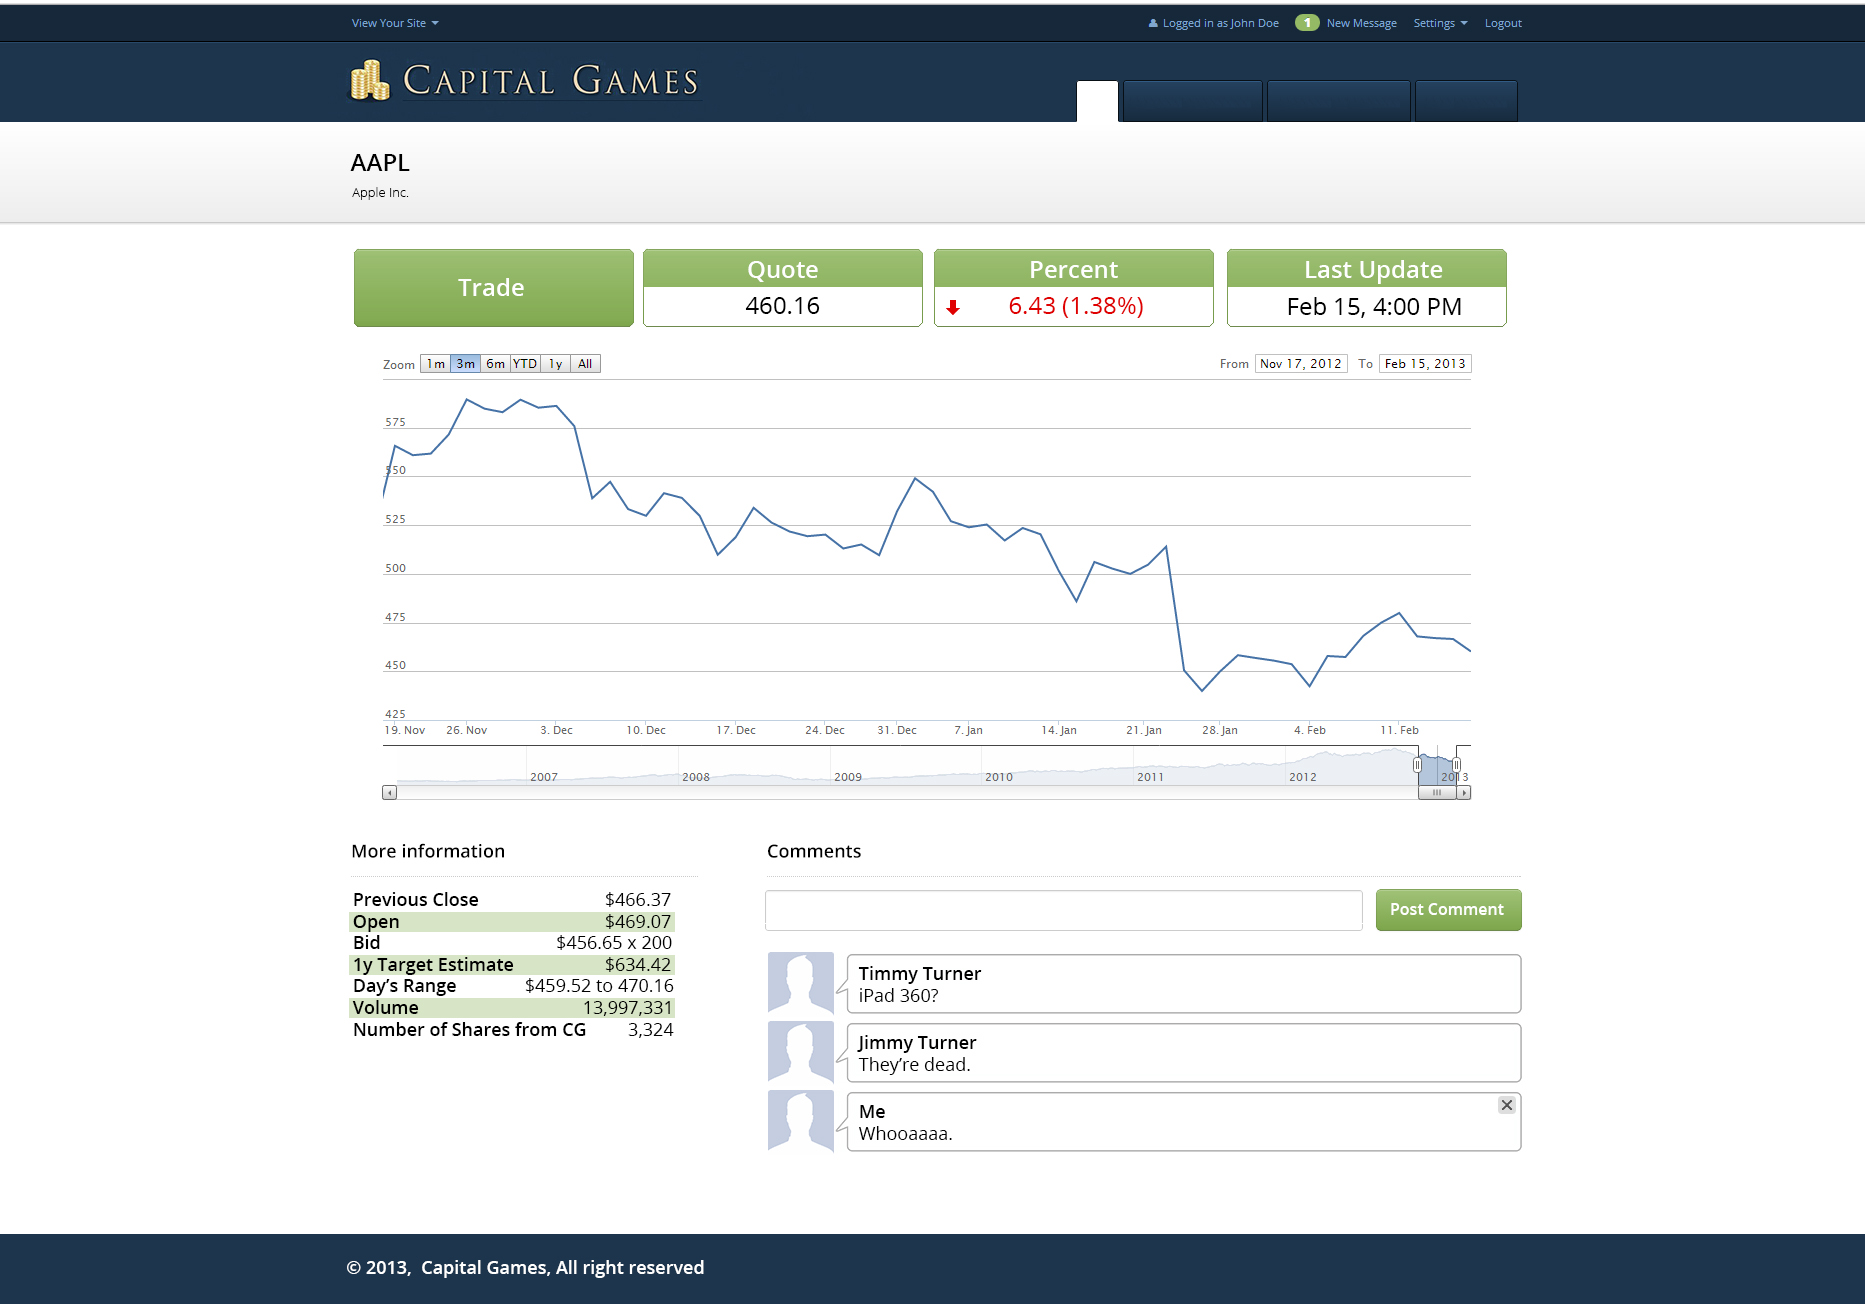
\includegraphics{./mockups/JPEG/company.jpg}
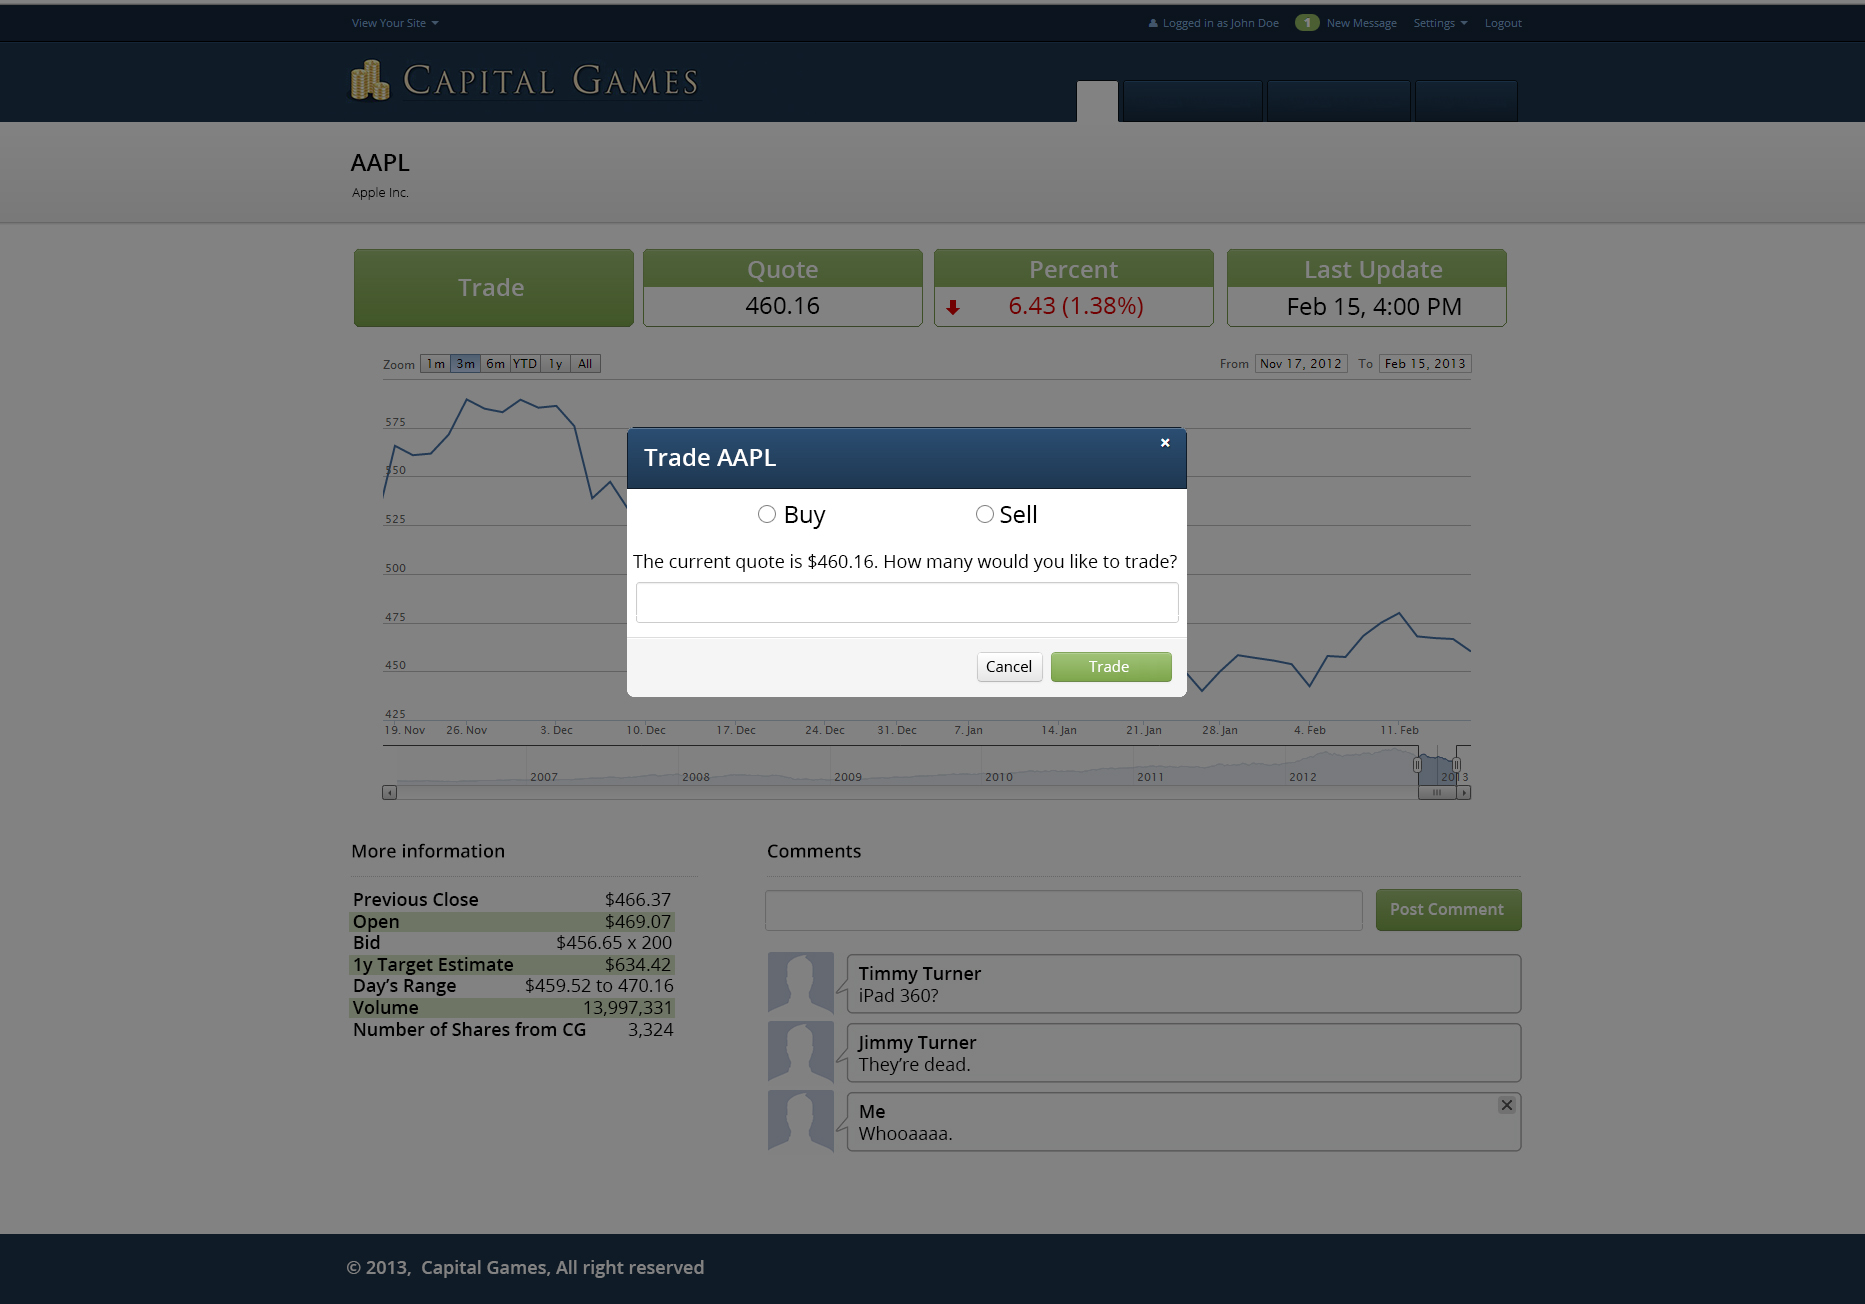
\includegraphics{./mockups/JPEG/Trade_popup.jpg}

\subsection{League}
From this page, you are able to view a certain league. Up at the top are the main facts about the league as well as a button to join/quit the league and the icon for it. In the middle, there is a ranking system to show the users in the highest standing. Down at the bottom, you can see the activity and also comment on the league itself. //
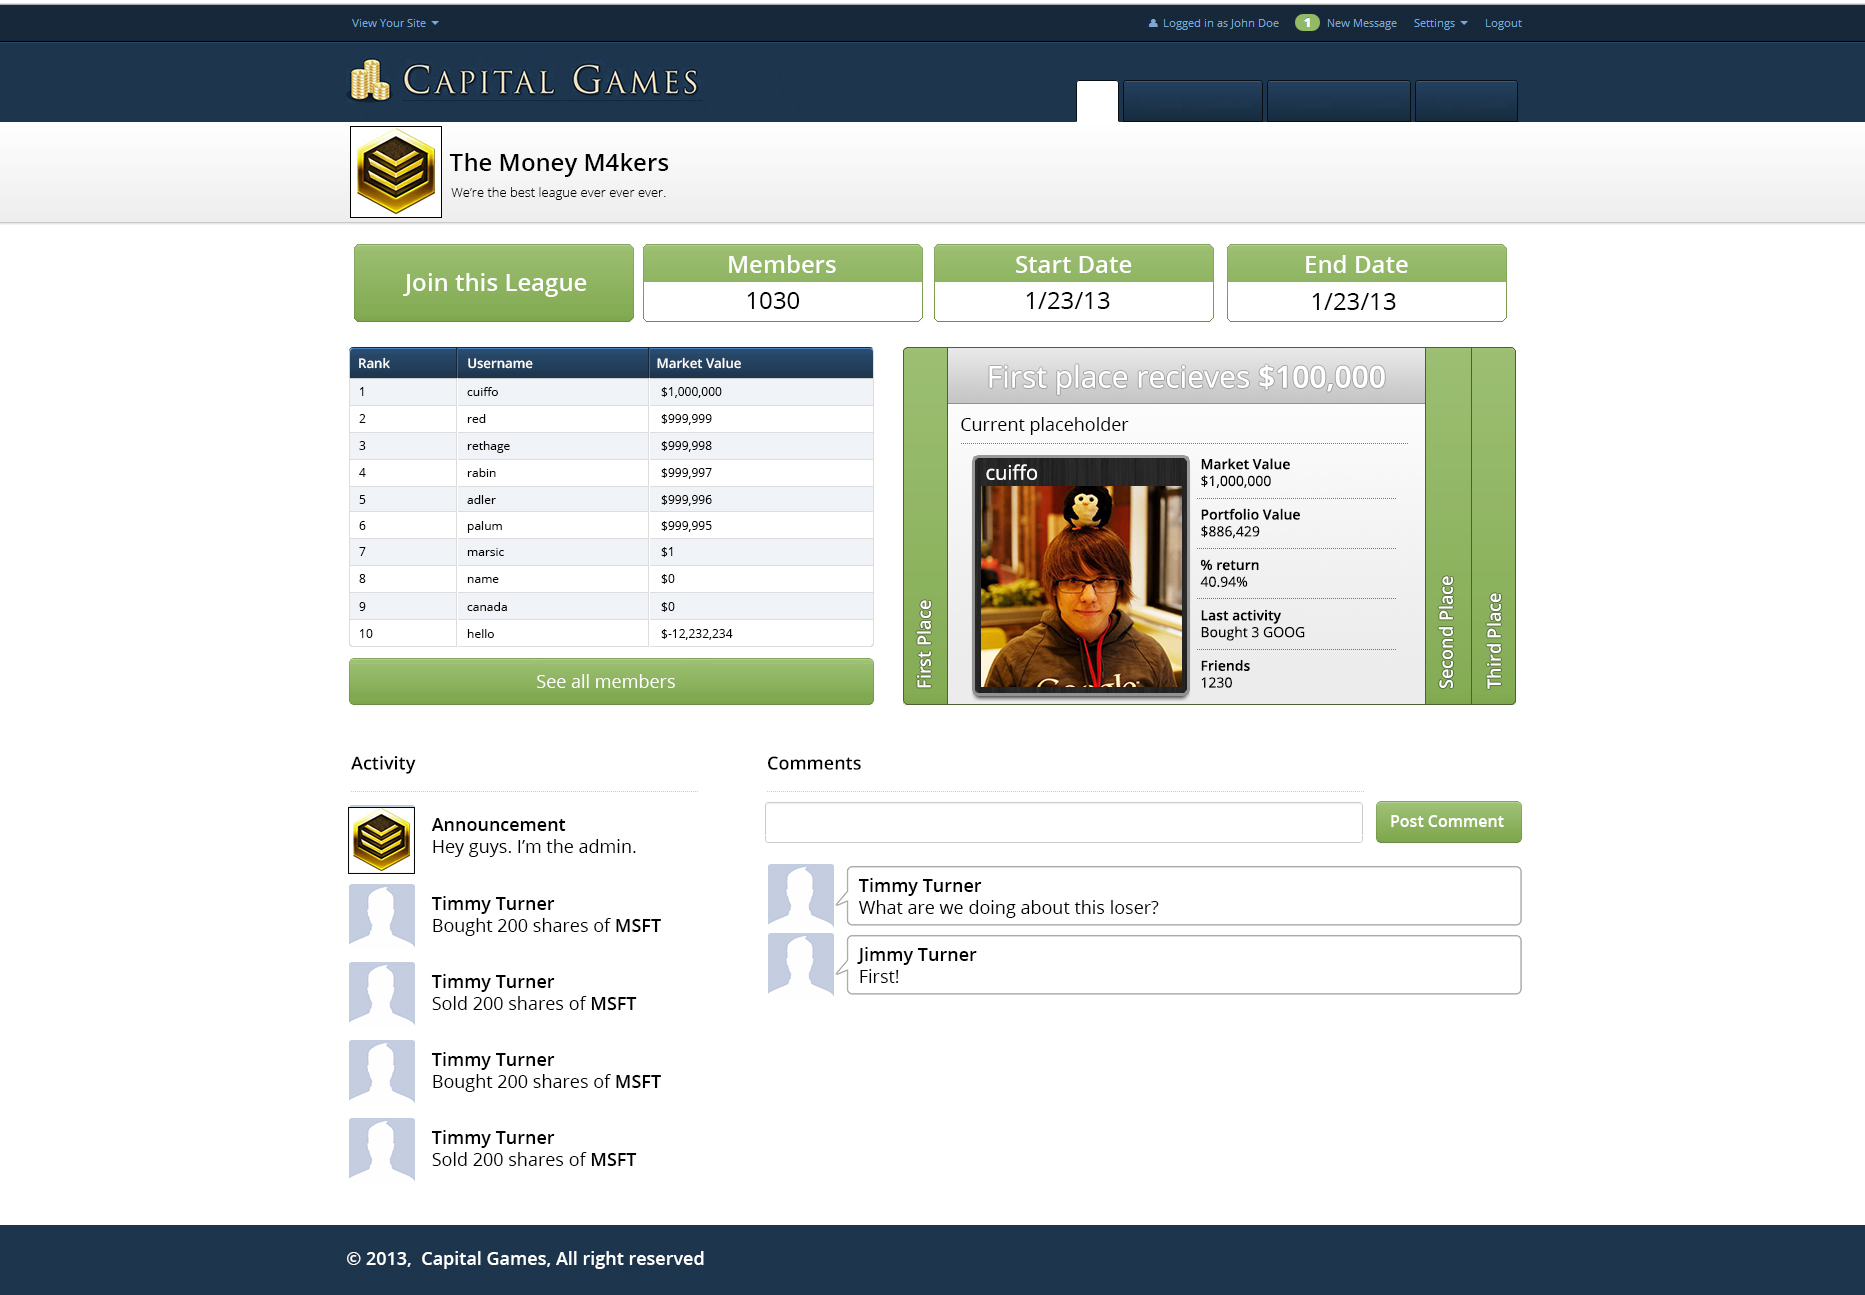
\includegraphics{./mockups/JPEG/Leagues_third.jpg}

\subsection{League Admin}
A league admin will see the join/quit button on a league as the settings page for them. When they click on that, they are brought to a page that gives them many settings they can change for the league, the most typical being the name, description and icon.//
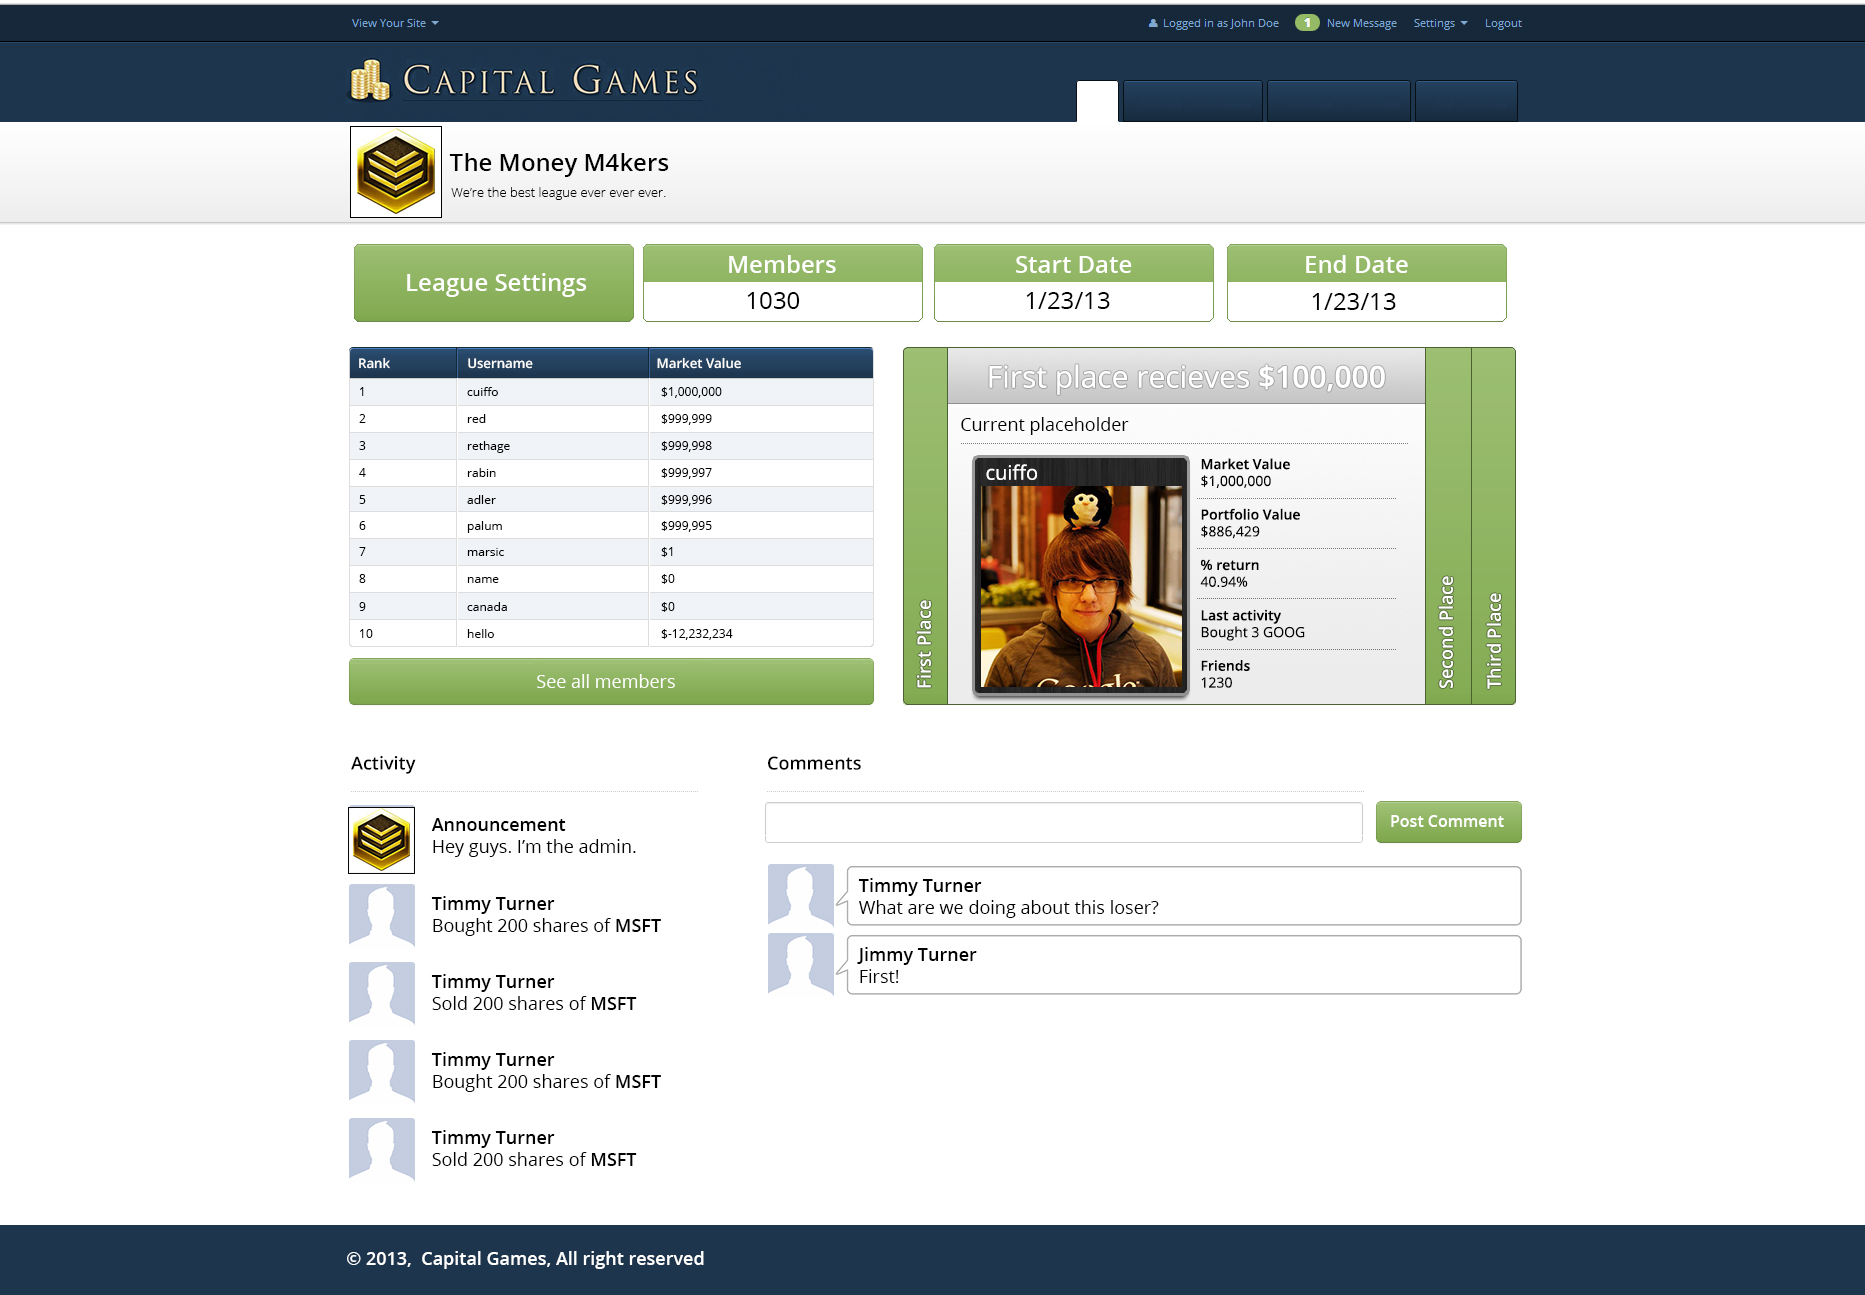
\includegraphics{./mockups/JPEG/Leagues_admin.jpg}
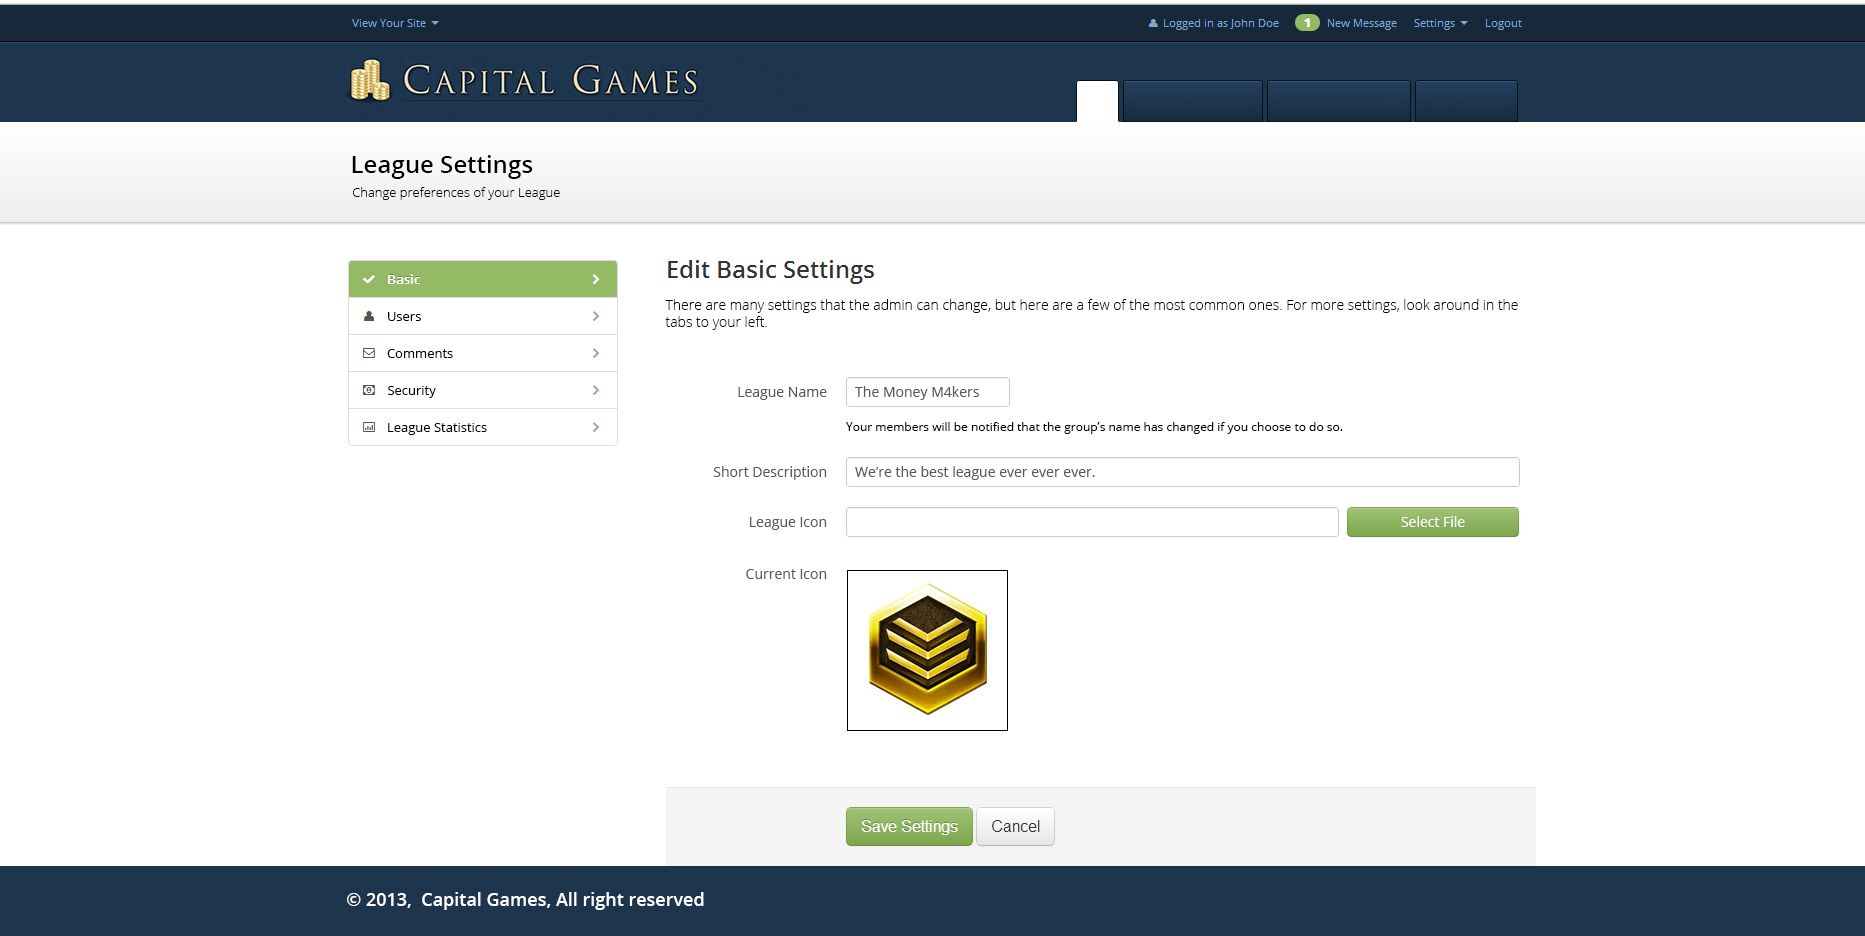
\includegraphics{./mockups/JPEG/league_admin.jpg}

\subsection{Messages}
A league admin will see the join/quit button on a league as the settings page for them. When they click on that, they are brought to a page that gives them many settings they can change for the league, the most typical being the name, description and icon.//
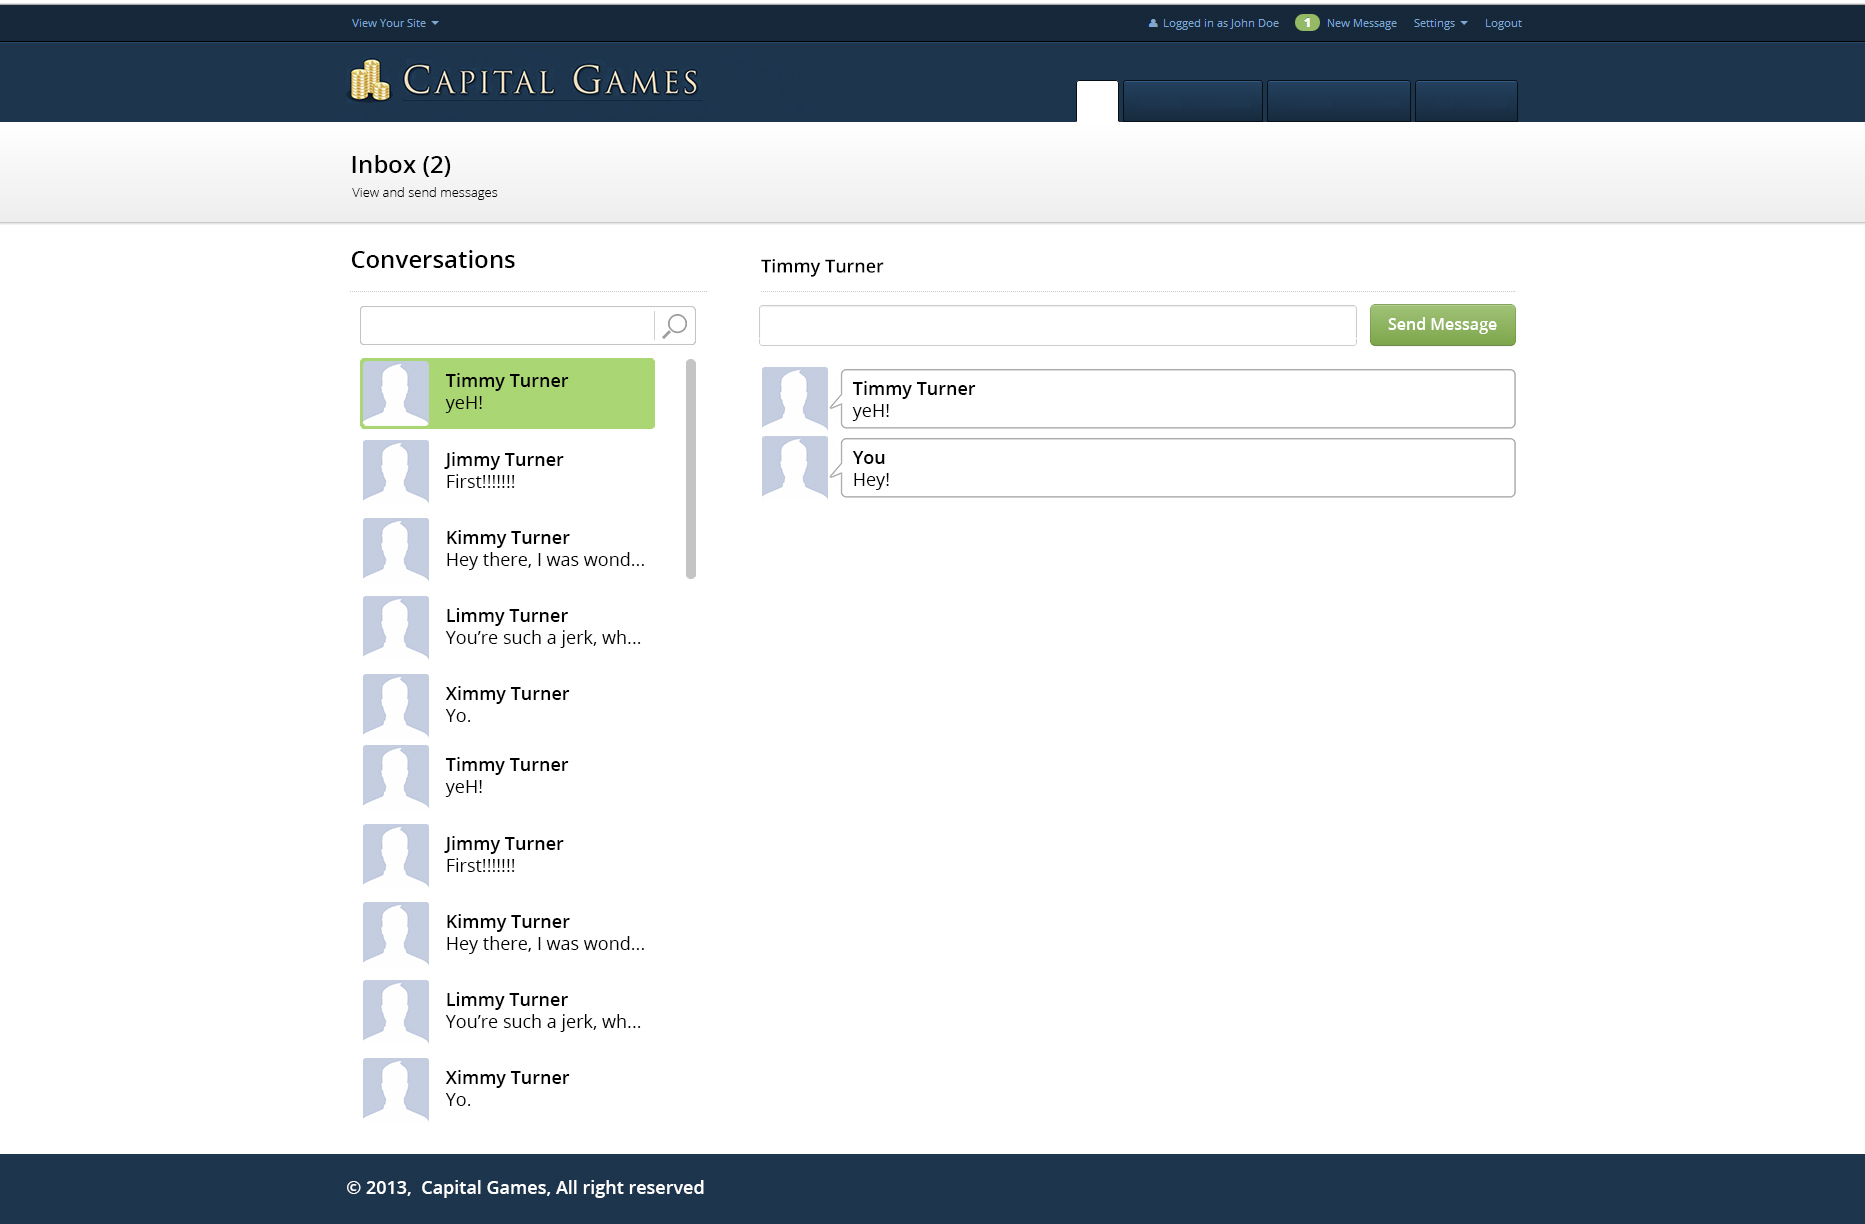
\includegraphics{./mockups/JPEG/messages.jpg}


% This section contains lots of explanations
% of user effort and ease of access
% See Appendix A for examples to boost grade
\section{User Effort Estimation}